\documentclass[tikz,border=10pt]{standalone}
\usepackage{tikz}
\usepackage{amsmath}
\usetikzlibrary{positioning, arrows.meta, calc}

\begin{document}
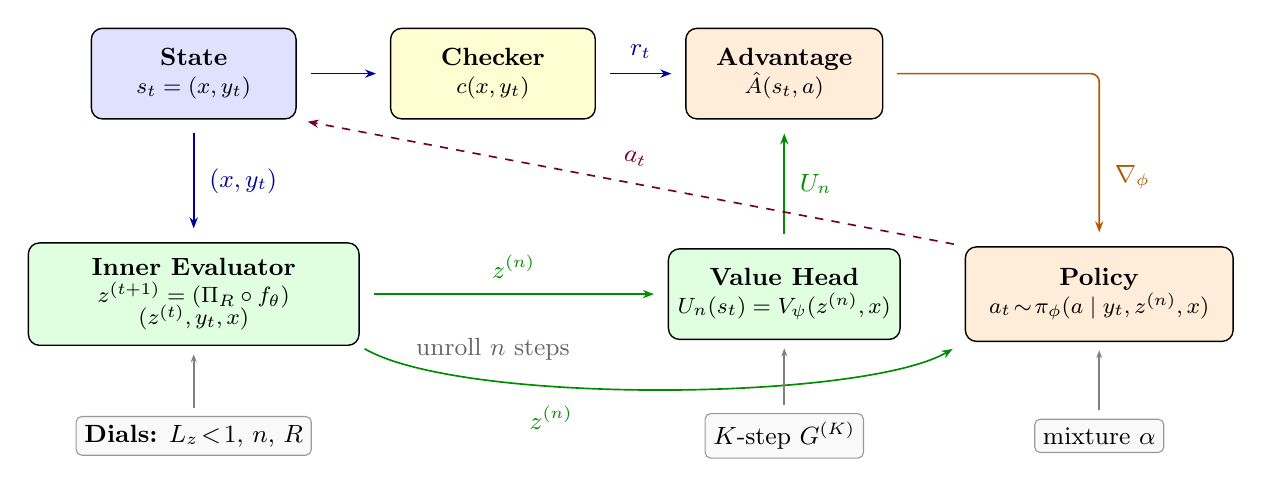
\begin{tikzpicture}[
    % Node styles - INCREASED SIZES (Fix A)
    mainbox/.style={
        draw, rounded corners=4pt, minimum height=1.15cm, minimum width=2.6cm,
        font=\small, align=center, thick, line width=0.5pt
    },
    % STRONGER FILL COLORS (Fix D)
    statebox/.style={mainbox, fill=blue!12},
    evalbox/.style={mainbox, fill=green!12},
    policybox/.style={mainbox, fill=orange!15},
    checkerbox/.style={mainbox, fill=yellow!18},
    % Arrow styles - INCREASED VISIBILITY (Fix D)
    arrow/.style={-{Stealth[scale=0.7]}, semithick, shorten >=5pt, shorten <=5pt},
    dataarrow/.style={arrow, blue!60!black},
    gradarrow/.style={arrow, orange!70!black},
    feedarrow/.style={arrow, green!55!black},
    actionarrow/.style={arrow, purple!60!black, dashed},
    % DARKER ANNOTATION STYLE (Fix D)
    lightarrow/.style={-{Stealth[scale=0.5]}, black!50, shorten >=3pt, shorten <=3pt, semithick},
    annotbox/.style={draw=black!40, fill=gray!5, rounded corners=2pt, font=\small, inner sep=3pt},
]

% ============================================================
% LAYOUT: 2-row grid
%   Top row (y=2.8):    State --- Checker --- Advantage
%   Bottom row (y=0):   Evaluator --------- ValueHead --- Policy
% ============================================================

% --- Top Row (y=2.8) ---
\node[statebox] (state) at (0, 2.8) {
    \textbf{State}\\[-1pt]
    {\footnotesize $s_t = (x, y_t)$}
};

\node[checkerbox] (checker) at (3.8, 2.8) {
    \textbf{Checker}\\[-1pt]
    {\footnotesize $c(x, y_t)$}
};

\node[policybox, minimum width=2.5cm] (adv) at (7.5, 2.8) {
    \textbf{Advantage}\\[-1pt]
    {\footnotesize $\hat{A}(s_t, a)$}
};

% --- Bottom Row (y=0) ---
% SPLIT EQUATION FOR READABILITY (Fix A)
\node[evalbox, minimum width=4.2cm, minimum height=1.3cm] (eval) at (0, 0) {
    \textbf{Inner Evaluator}\\[-1pt]
    {\footnotesize $z^{(t+1)} = (\Pi_R \circ f_\theta)$}\\[-3pt]
    {\footnotesize $(z^{(t)}, y_t, x)$}
};

% INCLUDE s_t EXPLICITLY (Fix A)
\node[evalbox, minimum width=2.8cm, minimum height=1.15cm] (vhead) at (7.5, 0) {
    \textbf{Value Head}\\[-1pt]
    {\footnotesize $U_n(s_t) = V_\psi(z^{(n)}, x)$}
};

\node[policybox, minimum width=3.4cm, minimum height=1.2cm] (policy) at (11.5, 0) {
    \textbf{Policy}\\[-1pt]
    {\footnotesize $a_t \!\sim\! \pi_\phi(a \mid y_t, z^{(n)}, x)$}
};

% ============================================================
% MAIN ARROWS - Clean routing, zero crossings
% ============================================================

% 1. State -> Checker (horizontal, top row)
\draw[dataarrow] (state.east) -- (checker.west);

% 2. Checker -> Advantage (horizontal, top row, with reward label)
\draw[dataarrow] (checker.east) -- node[above=2pt, font=\small] {$r_t$} (adv.west);

% 3. State -> Evaluator (vertical, left column)
\draw[dataarrow] (state.south) -- node[right=2pt, font=\small, pos=0.5] {$(x, y_t)$} (eval.north);

% 4. Evaluator -> Value Head (horizontal, bottom row)
\draw[feedarrow] (eval.east) -- node[above=2pt, font=\small, pos=0.5] {$z^{(n)}$} (vhead.west);

% 5. Value Head -> Advantage (vertical)
\draw[feedarrow] (vhead.north) -- node[right=2pt, font=\small, pos=0.5] {$U_n$} (adv.south);

% 6. Advantage -> Policy (orthogonal: right at y=2.8, then down to policy.north)
%    This frees policy.west for the z->policy arrow and avoids all crossings
\draw[gradarrow, rounded corners=3pt]
    (adv.east) -- (11.5, 2.8) -- (policy.north)
    node[pos=0.6, right=2pt, font=\small] {$\nabla_\phi$};

% 7. Evaluator -> Policy (policy conditions on z^{(n)}, curved path)
%    Route: from eval.south east curving to policy.south west
\draw[feedarrow, shorten <=2pt]
    (eval.south east) to[out=-30, in=-150, looseness=0.5]
    node[below=4pt, font=\small, pos=0.35] {$z^{(n)}$}
    (policy.south west);

% 8. Policy -> State: ACTION ARROW (straight diagonal)
%    Clear visual that action comes from Policy and updates State
\draw[actionarrow, shorten >=4pt, shorten <=4pt]
    (policy.north west) -- (state.south east)
    node[above=3pt, font=\small, pos=0.5, sloped] {$a_t$};

% ============================================================
% ANNOTATIONS - DARKER AND MORE VISIBLE (Fix D)
% ============================================================

% n steps label (between Evaluator and Value Head)
\node[font=\small, black!60] at (3.8, -0.7) {unroll $n$ steps};

% K-step bootstrap (below Value Head)
\node[annotbox] (kstep) at (7.5, -1.8) {$K$-step $G^{(K)}$};
\draw[lightarrow] (kstep.north) -- (vhead.south);

% Conservative mixture alpha (below Policy)
\node[annotbox] (alpha) at (11.5, -1.8) {mixture $\alpha$};
\draw[lightarrow] (alpha.north) -- (policy.south);

% TRM Dials (below Evaluator)
\node[annotbox] (dials) at (0, -1.8) {\textbf{Dials:} $L_z\!<\!1$, $n$, $R$};
\draw[lightarrow] (dials.north) -- (eval.south);

\end{tikzpicture}
\end{document}
